% generated by scripts/pkl_to_latex.py
% source PKL : uscan_v1_L6_Ne6_t0p1_mode-uniform_nmin2_solver-gcg_full_restarts8_iter300_kmax2_tol1em09_U0to15_N16-2f7c06936fa2.pkl
% scan type  : uscan
% state      : gs
% quantity   : linear-entropy
% requires   : \usepackage{pgfplots} \pgfplotsset{compat=1.18}
% colours match the matplotlib PDF (tab10 cycle)
\definecolor{gmeC0}{HTML}{1F77B4}
\definecolor{gmeC1}{HTML}{FF7F0E}
\definecolor{gmeC2}{HTML}{2CA02C}
\definecolor{gmeC3}{HTML}{D62728}
\definecolor{gmeC4}{HTML}{9467BD}
\definecolor{gmeC5}{HTML}{8C564B}
\definecolor{gmeC6}{HTML}{E377C2}
\definecolor{gmeC7}{HTML}{17BECF}

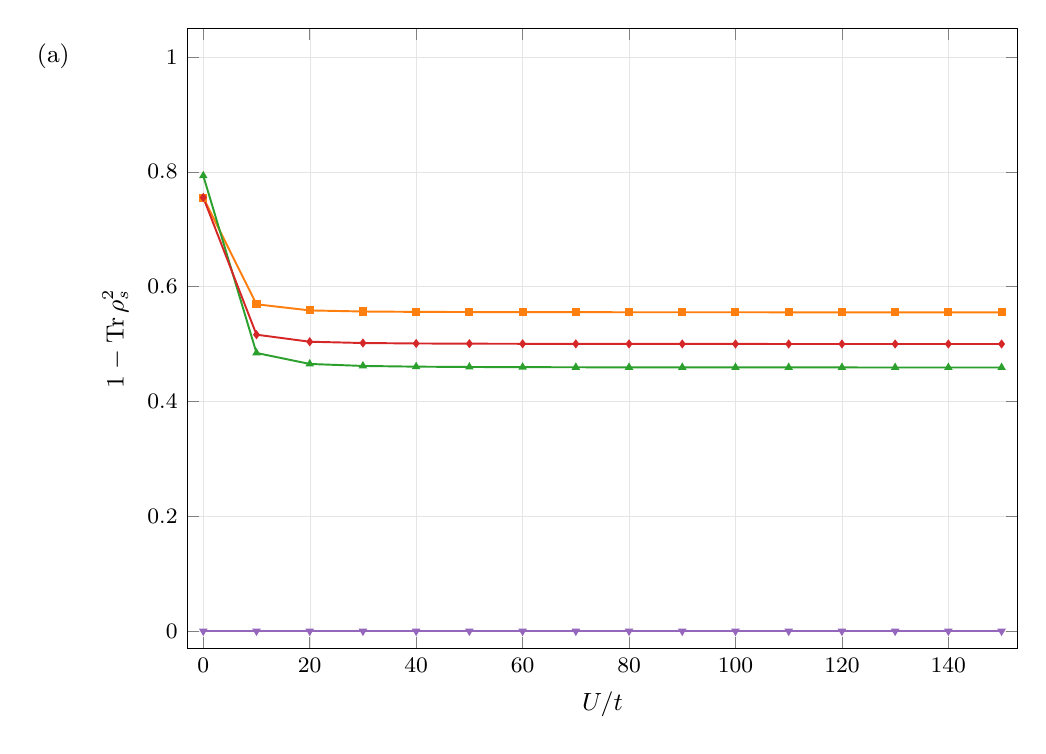
\begin{tikzpicture}
  \begin{axis}[
    width=\columnwidth,
    height=0.78\columnwidth,
    xlabel={$U/t$},
    ylabel={$1-\mathrm{Tr}\,\rho_s^2$},
    grid=both,
    grid style={line width=.1pt, draw=gray!20},
    tick label style={font=\footnotesize\rmfamily, /pgf/number format/fixed},
    label style={font=\small\rmfamily},
    scaled ticks=false,
    legend style={font=\scriptsize\rmfamily, draw=gray!40, at={(0.5,1.03)}, anchor=south, /tikz/every even column/.append style={column sep=6pt}},
    legend cell align={left},
    legend columns=2,
    ymin=-0.03,
    ymax=1.05,
    xmin=-3,
    xmax=153,
    after end axis/.append code={\node[anchor=east, font=\small\rmfamily] at (axis description cs:-0.13,0.954) {(a)};},
  ]
    \addplot[color=gmeC1, mark=square*, mark size=1.1pt, line width=0.7pt] coordinates {
        (0,0.755) (10,0.569263) (20,0.558565) (30,0.55669)
        (40,0.55604) (50,0.55574) (60,0.555577) (70,0.555479)
        (80,0.555415) (90,0.555372) (100,0.55534) (110,0.555317)
        (120,0.5553) (130,0.555286) (140,0.555275) (150,0.555267)
    };
    \addplot[color=gmeC2, mark=triangle*, mark size=1.1pt, line width=0.7pt] coordinates {
        (0,0.793091) (10,0.484489) (20,0.465366) (30,0.461862)
        (40,0.460634) (50,0.460065) (60,0.459756) (70,0.45957)
        (80,0.459449) (90,0.459366) (100,0.459307) (110,0.459263)
        (120,0.459229) (130,0.459203) (140,0.459183) (150,0.459166)
    };
    \addplot[color=gmeC3, mark=diamond*, mark size=1.1pt, line width=0.7pt] coordinates {
        (0,0.755198) (10,0.516315) (20,0.504049) (30,0.501801)
        (40,0.501013) (50,0.500649) (60,0.500451) (70,0.500331)
        (80,0.500254) (90,0.5002) (100,0.500162) (110,0.500134)
        (120,0.500113) (130,0.500096) (140,0.500083) (150,0.500072)
    };
    \addplot[color=gmeC4, mark=triangle*, mark size=1.1pt, mark options={rotate=180}, line width=0.7pt] coordinates {
        (0,0) (10,0) (20,-0) (30,0)
        (40,0) (50,-0) (60,0) (70,0)
        (80,0) (90,0) (100,0) (110,0)
        (120,-0) (130,-0) (140,0) (150,-0)
    };
  \end{axis}
\end{tikzpicture}
